\documentclass[a4paper,10pt]{article}

\usepackage{ucs}
\usepackage[utf8]{inputenc}
\usepackage{float}
\usepackage{babel}
\usepackage{fontenc}
\usepackage{graphicx}

\usepackage[dvips]{hyperref}
\renewcommand{\familydefault}{\sfdefault}

\title{Report Interactive Graphics Project
}
\date{26/2/19}
\author{%
\newline Teacher: Marco Schaerf\\
Author: Federico Bacci\\
}

\begin{document}

\maketitle
\pagenumbering{gobble}


\iffalse \newpage \fi
\pagenumbering{arabic}

\begin{figure}[H]
  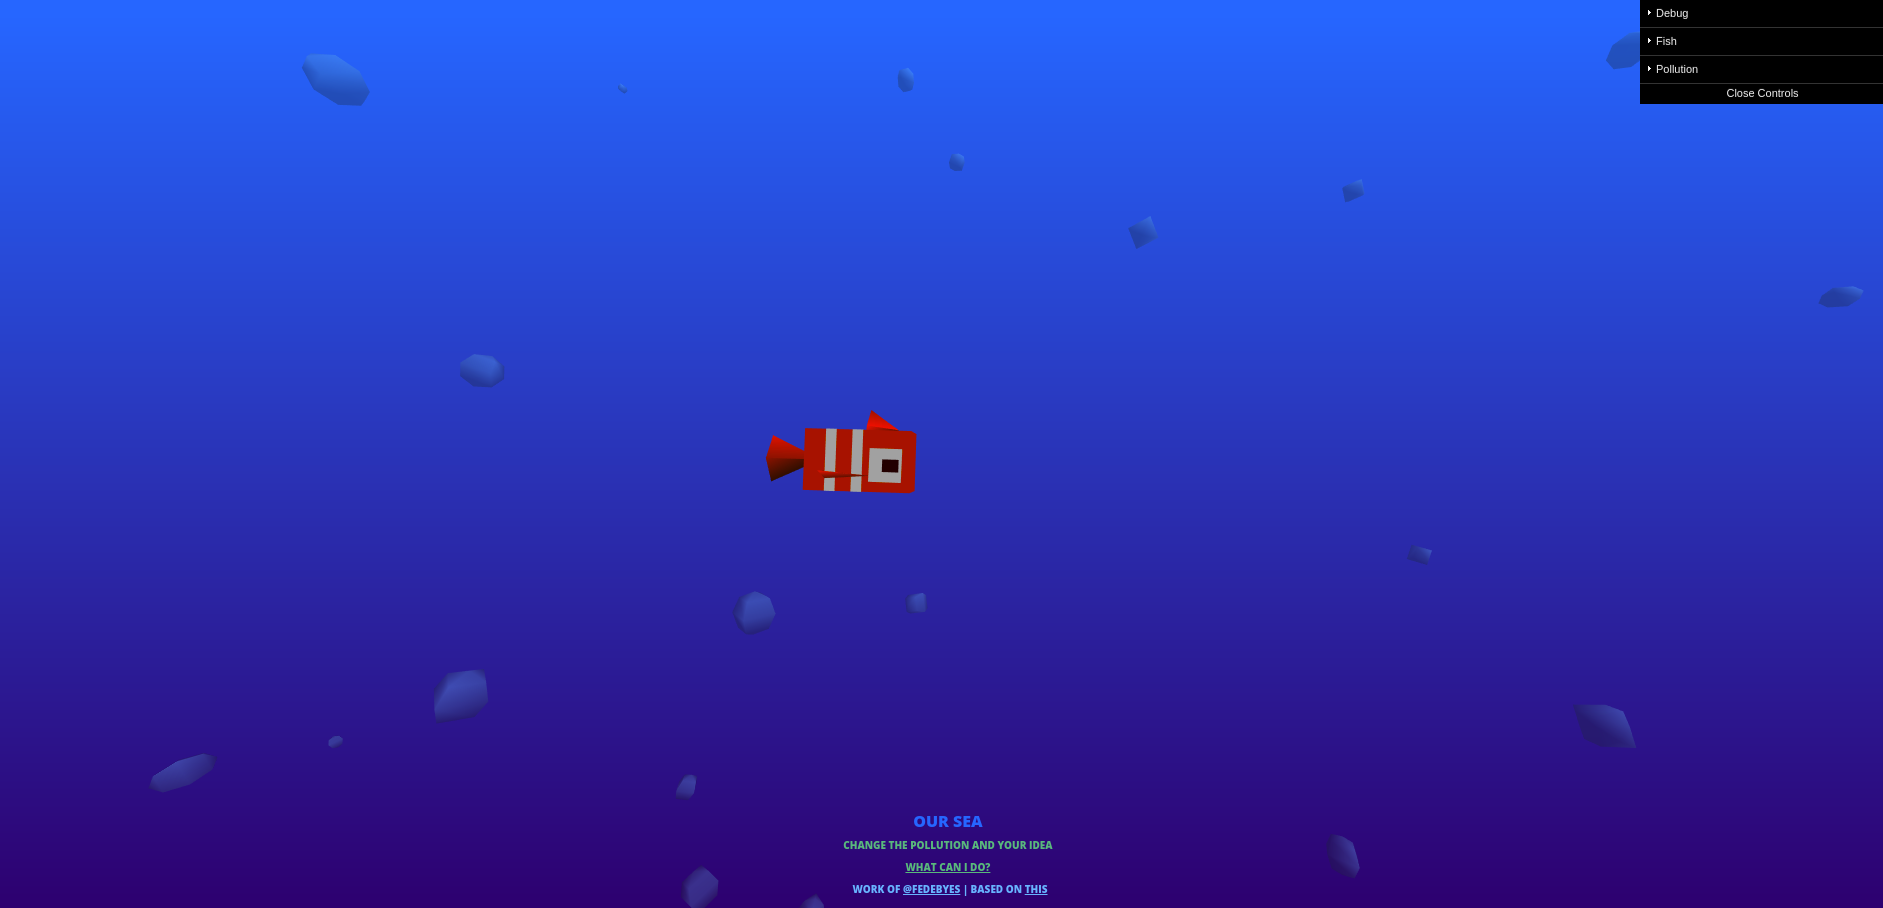
\includegraphics[width=\linewidth]{Screenshot_20190226_181608.png}
\end{figure}
{\center {\huge 
Our Sea\\ \\ Change the pollution and your idea}
\newpage}}

\section{Introduction}

 The idea for this project comes from the need to inform and inspire on the Issue of plastic pullution in {\bf Our Sea}. It is pointed out from numerous articles that every year 8 million of metric tons of plastic are thrown awain into the ocean.

The main character is a small fish that is swimming in the ocean, as we change the pollution of the ocean the fish become gradually sicker and sad.


\section{Environment}

To develop the application I used the {\bf Three.js} library. Preferred over {\bf Web GL} standard library because the large level of abstraction and customization.
Also in the project were used different libraries of Javascript here is the complete list:

\begin{itemize}
 \item {\bf Three.js} to create an easy to use, lightweight, 3D library. The library provides Canvas 2D, SVG, CSS3D and WebGL renderers.
 \item {\bf OrbitControls.js}  part of the Three.js Project to control the camera with the mouse
 \item {\bf Math.js} for the mathematical computation in the project
 \item {\bf Stats.js} part of Three.js Project to check the Frames per Second (FPS)
 \item {\bf Dat.GUI.js} part of Three.js Project to create an easy gui to edit parameters
\end{itemize}


\section{Techical Aspects}

\subsection{HTML}
\begin{figure}[H]
  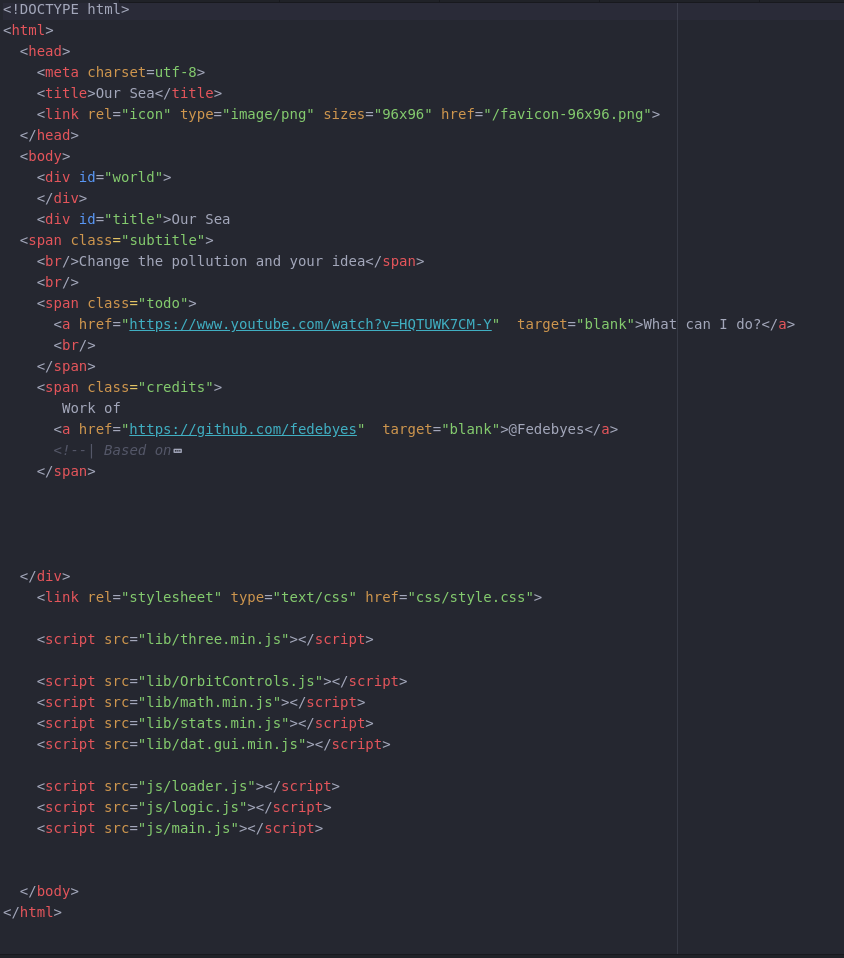
\includegraphics[width=\linewidth]{Screenshot_20190226_185740.png}
\end{figure}



The HTML file contains just the title and the Javascript libraries that we have listed plus the files that we have created for the project




\subsection{CSS}
\begin{figure}[H]
  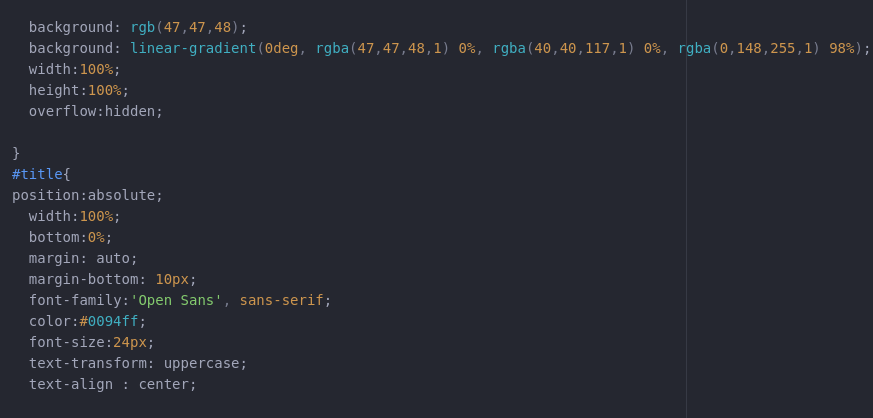
\includegraphics[width=\linewidth]{Screenshot_20190226_190022.png}
\end{figure}
In the file style.css are contained just the information for the background and the title styling

\subsection{Javascript}

The Javascript code is divided in 3 files
\begin{itemize}
 \item loader.js
 \item logic.js
 \item main.js
\end{itemize}

\subsubsection{main.js}
\begin{figure}[H]
  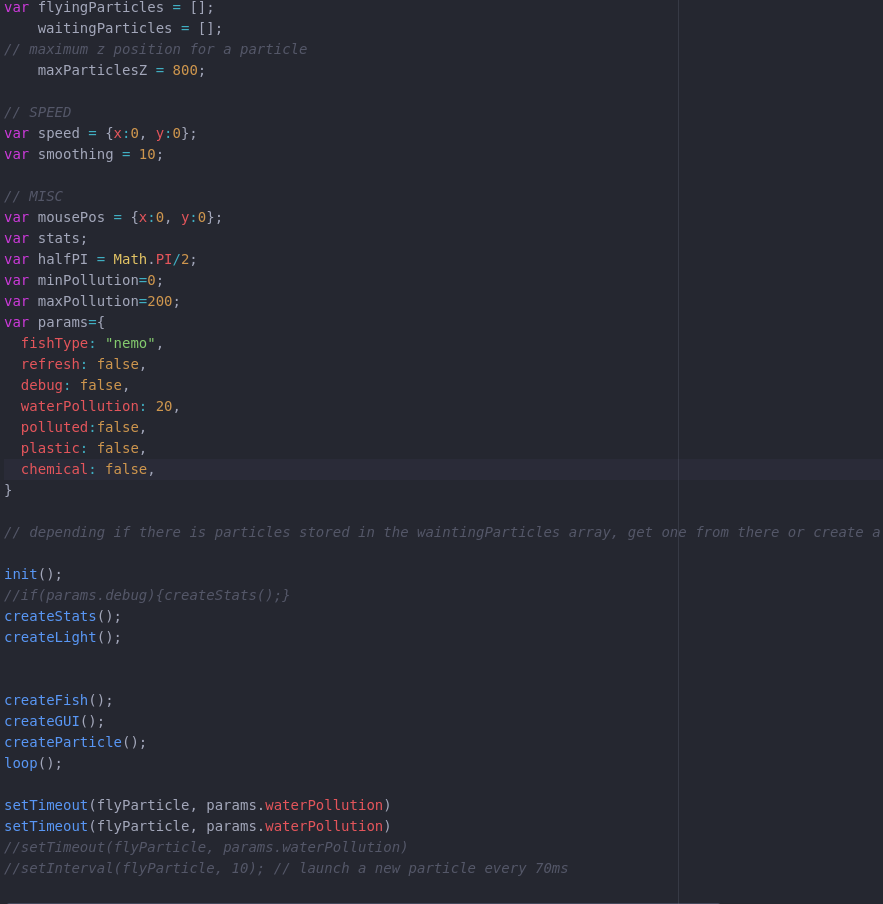
\includegraphics[width=\linewidth]{Screenshot_20190226_190629.png}
\end{figure}
In this file all variables are defined, including scene, camera, container and renderer. 
After that custom variables are defined like colors and speed.



\subsubsection{loader.js}
\begin{figure}[H]
  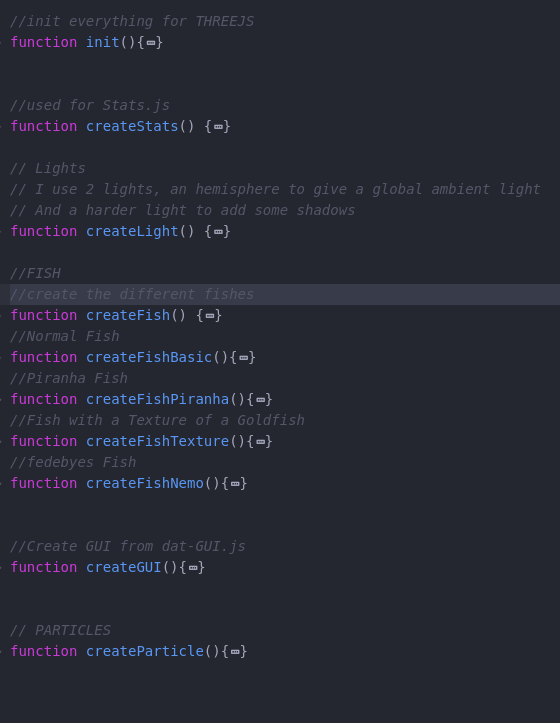
\includegraphics[width=\linewidth]{Screenshot_20190226_191007.png}
\end{figure}
The javascript function of this file are necessary to load the Environment.


\begin{itemize}
 \item {\bf init()} Creates a scene, the camera, the renderer and add all listeners to the document
 \item {\bf createStats()} Creates the Stats for Stats.js
 \item {\bf createLight()} add lights to the scene one HemispereLight and one DirectionalLight
 \item {\bf createFish()} is in charge of creating the fish, generally composed of a lot of polygons
 \item {\bf createFishbasic()} create a cube for the body of the fish then a MeshLambertMaterial is added, the tail is a CylinderGeometry, like all the fins, while the eyes are a BoxGeometry as the iris
 \item {\bf createFishPiranha()} is the same as createFish() just with the adds of a different colour and the teeth of the fish that are another BoxGeometry
 \item {\bf createFishTexture()} is the same as createFishBasic() just with the add of a Goldfish Texture image
 \item {\bf createFishNemo()} creates a Red fish with big eyes like the Nemo cartoon, easy to impersonate swimming in the ocean
 \item {\bf createGUI()} is the function that adds the GUI to the project to change variables, using the library dat.GUI.js
 \item {\bf createParticle()} Creates different types of particles with random colors, scale and dimensions.
 \begin{itemize}
 \item The Bubble particles are a Sphere geomety with a transparent MeshLambertMaterial.
 \item The Plastic particles are BoxGeometry.
 \item The Dirt particles are SphereGeometry.
 \item The Chemical particles are TetrahedronGeometry.
 \end{itemize}
\end{itemize}




\subsubsection{logic.js}
\begin{figure}[H]
  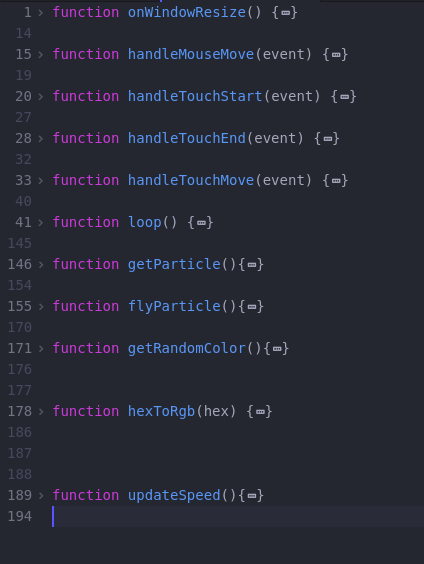
\includegraphics[width=\linewidth]{Screenshot_20190226_192414.png}
\end{figure}
This was the most difficult part of the project with countless of mathematical function to operate all the animations.




\begin{itemize}
 \item {\bf  onWindowResize()} Handles the event for window resizing
 \item {\bf handleMouseMove(event)} handle the event for touch moving
 \item {\bf handleTouchStart(event)} handle the event for touch start
 \item {\bf handleTouchEnd(event)} handle the event for touch end
 \item {\bf handleTouchMove(event)} handle the event for touch moving so is compatible also with the phone
 \item {\bf loop()} the most complicated part of the project, this is the also called requestAnimationFrame.
 Based on the purity of the water it change the color of the fish, while based on the speed it change the scale to let struggle the fish when the mouse is on the right and making a calm pose when the mouse is on the left.
 Depending on the mouse position the eyes of the fish and the body follow the mouse so we can see it in 3D.
 This function also let move the fins of the fish with a mathematical function of cosen for the rotation of the tail, leftFin, rightFin and topFin.
 \item {\bf getParticle()}
 \item {\bf flyParticle()} let particles move simulating a current
 \item {\bf getRandomColor()} get a color from the random color that we created
 \item {\bf hexToRgb(hex)} is used to create a RGB color type from an HEX one
 \item {\bf updateSpeed()} update the speed according the mouse position
 
 
 
 
 
 
\end{itemize}



\subsection{Components}


\subsubsection{Scene}
\begin{figure}[H]
  
\includegraphics[width=\linewidth]{Screenshot_20190226_195128.png}
\end{figure}
The scene is nothing more than a background with two lights added, a HemispereLight and a DirectionalLight.

\subsubsection{Particles}

\begin{figure}[H]
    \centering
    \begin{minipage}{0.45\textwidth}
        \centering
        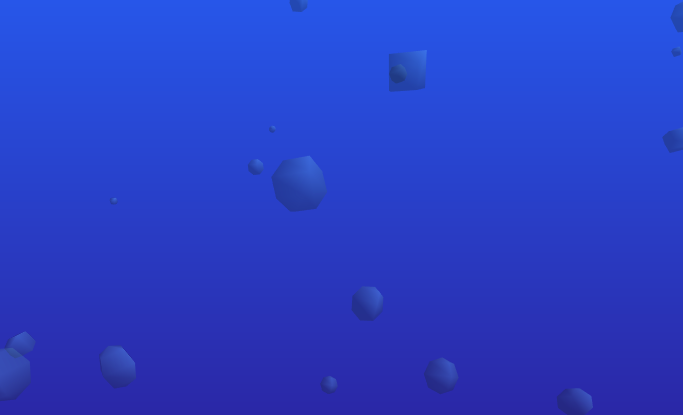
\includegraphics[width=1\textwidth]{Screenshot_20190226_200209.png} % first figure itself
        \caption{Bubble Particles}
    \end{minipage}\hfill
    \begin{minipage}{0.45\textwidth}
        \centering
        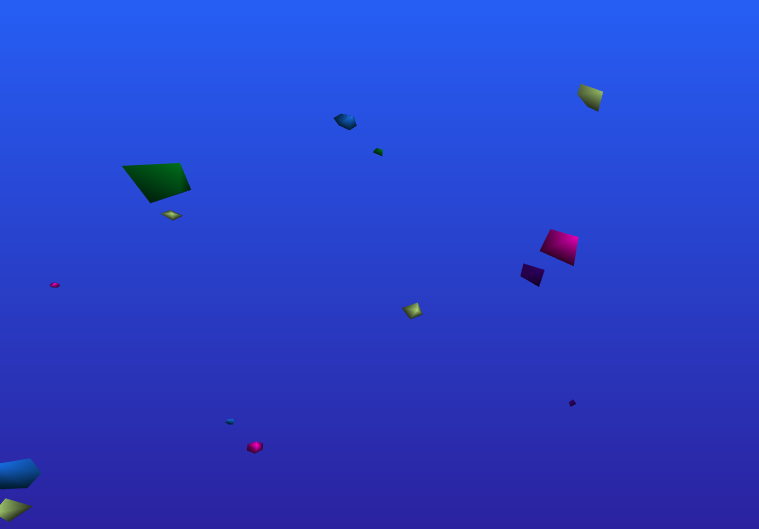
\includegraphics[width=1\textwidth]{Screenshot_20190226_200304.png} % second figure itself
        \caption{Dirt Particles}
    \end{minipage}
\end{figure}


\begin{figure}[H]
    \centering
    \begin{minipage}{0.45\textwidth}
        \centering
        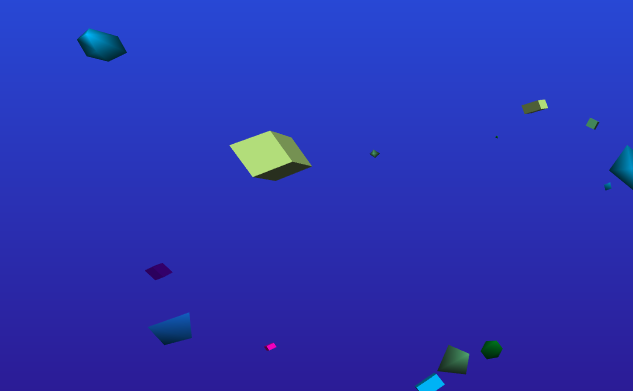
\includegraphics[width=1\textwidth]{Screenshot_20190226_200345.png} % first figure itself
        \caption{Plastic Particles}
    \end{minipage}\hfill
    \begin{minipage}{0.45\textwidth}
        \centering
        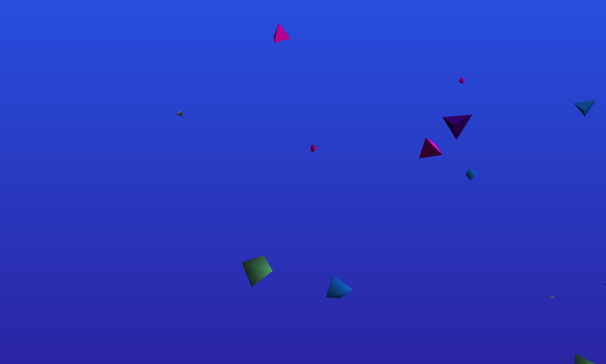
\includegraphics[width=1\textwidth]{Screenshot_20190226_200422.png} % second figure itself
        \caption{Chemical Particles}
    \end{minipage}
\end{figure}


These are the different particles that float into the sea, if it is not polluted and the Water Purity is high there are just oxygen bubbles, but if it is polluted the plastic, dirt and chemical partiles start to float around.




\subsubsection{Fish}


\begin{figure}[H]
    \centering
    \begin{minipage}{0.45\textwidth}
        \centering
        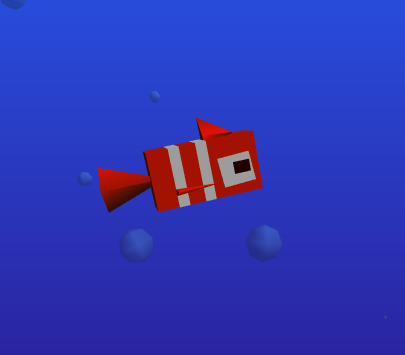
\includegraphics[width=1\textwidth]{Screenshot_20190226_200844.png} % first figure itself
        \caption{Nemo Fish}
    \end{minipage}\hfill
    \begin{minipage}{0.45\textwidth}
        \centering
        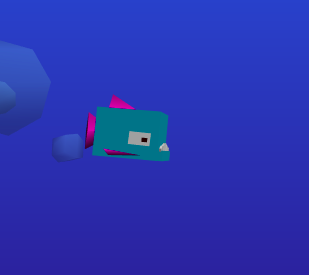
\includegraphics[width=1\textwidth]{Screenshot_20190226_200918.png} % second figure itself
        \caption{Piranha Fish}
    \end{minipage}
\end{figure}


\begin{figure}[H]
    \centering
    \begin{minipage}{0.45\textwidth}
        \centering
        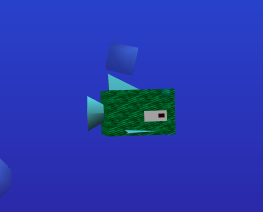
\includegraphics[width=1\textwidth]{Screenshot_20190226_201004.png} % first figure itself
        \caption{Texture Fish}
    \end{minipage}\hfill
    \begin{minipage}{0.45\textwidth}
        \centering
        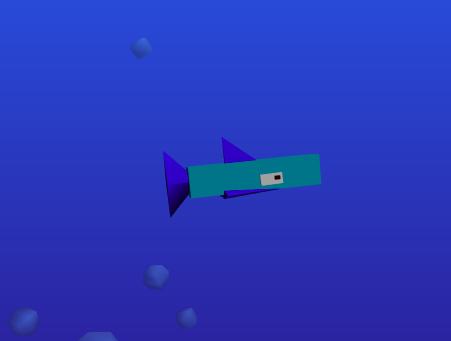
\includegraphics[width=1\textwidth]{Screenshot_20190226_201047.png} % second figure itself
        \caption{Normal Fish}
    \end{minipage}
\end{figure}

There are four different types of fish and each one of them interact differently with the colors and the pollution of the water.

Every fish is different but in general they are composed by

\begin{itemize}
 \item {\bf  Body} a BoxGeometry with a MeshLambertMaterial
 \item {\bf  Spot} two BoxGeometry with MeshLambertMaterial with a little distance from the body that is the parent
 \item {\bf  Tail} a CylinderGeometry with a MeshLambertMaterial scaled to resemble better a tail depending from the body
 \item {\bf Fin} two fin for lef and rigth that are Tails rotated for that
 \item {\bf  Top Fin} another fin very similar to the tail that is scaled and half of it is hidden in the body of the fish 
 \item {\bf  Eye} two BoxGeometry that are the Eyes of the fish, their parent is the body
 \item {\bf Iris} two BoxGeometry with a MeshLambertMaterial

\end{itemize}

\begin{figure}[H]
  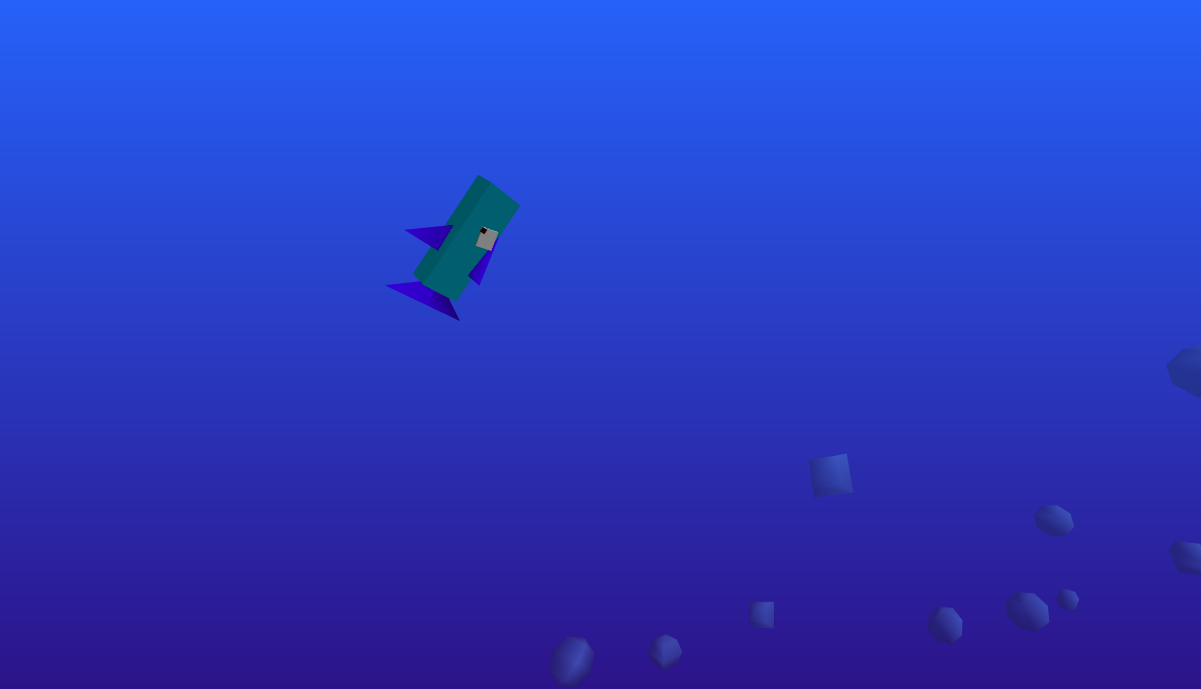
\includegraphics[width=\linewidth]{Screenshot_20190226_203131.png}
\end{figure}





\subsection{Interaction}
The main part of the project is the interaction, the user can move the mouse (or thouch on the smartphone) on the left or right and the fish will swim slower or faster respectively, scaling the parts and the body to simulate the movement.


\begin{figure}[H]
    \centering
    \begin{minipage}{0.45\textwidth}
        \centering
        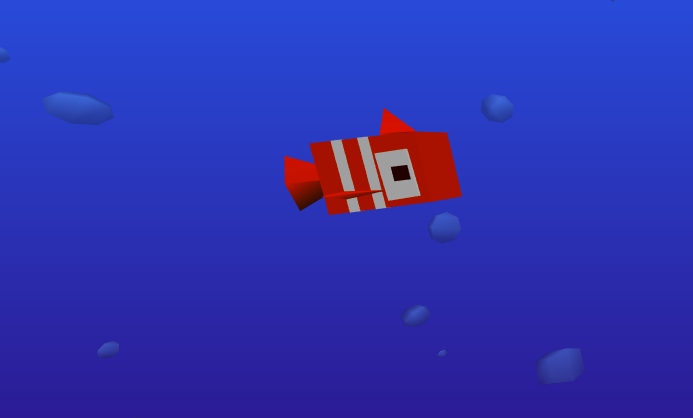
\includegraphics[width=1\textwidth]{Screenshot_20190226_202521.png} % first figure itself
        \caption{Calm Fish}
    \end{minipage}\hfill
    \begin{minipage}{0.45\textwidth}
        \centering
        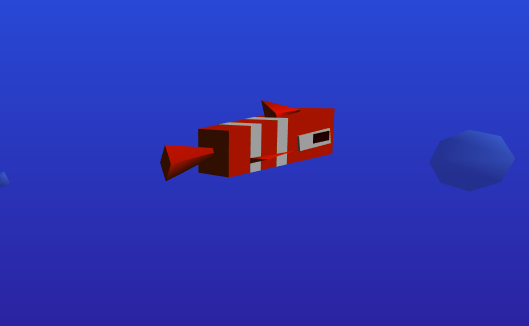
\includegraphics[width=1\textwidth]{Screenshot_20190226_202616.png} % second figure itself
        \caption{Swimming Fish}
    \end{minipage}
\end{figure}


Depending on the pollution the fish could be sane and sick, changing color.

\begin{figure}[H]
    \centering
    \begin{minipage}{0.45\textwidth}
        \centering
        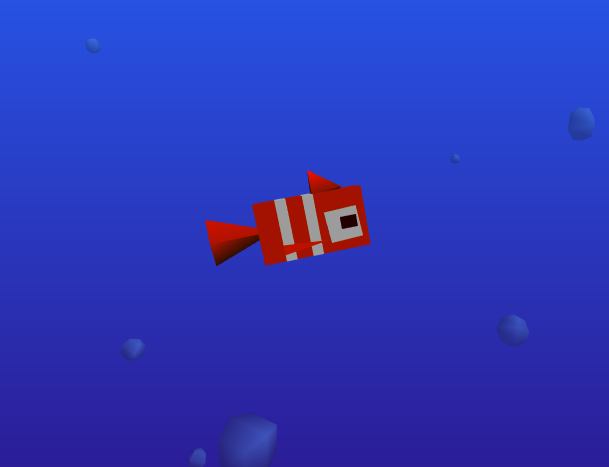
\includegraphics[width=1\textwidth]{Screenshot_20190226_202824.png} % first figure itself
        \caption{Sane Fish}
    \end{minipage}\hfill
    \begin{minipage}{0.45\textwidth}
        \centering
        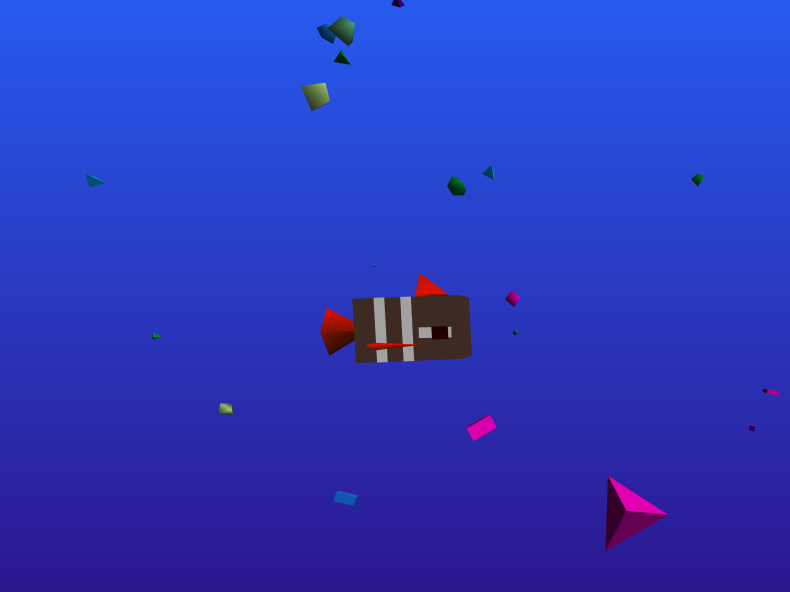
\includegraphics[width=1\textwidth]{Screenshot_20190226_202756.png} % second figure itself
        \caption{Sick Fish}
    \end{minipage}
\end{figure}

In the end the fish also can be moved with the mouse and the eyes will follow it using the different functions.



\subsection{Conclusion}

This project was aimed to understand and use in a real environment the WebGL technologies to create a Graphic that could be Interactive.
I think I have learned a lot on the technology creating a project that can be useful for something, the project is currently hosted on  \href{https://fedebyes.github.io/our-sea/}{fedebyes.github.io/our-sea}.
I've decided to call this project Our Sea to make people aware of the impact of pollution on our sea. 
\\
\\
\\
\\
\\
\\
{\center \Huge``We forget that water cycle and life cycle are one``\\
\hspace*{\fill}-Jaques Yves Cousteau}
\end{document}

